\documentclass{beamer}
% \usepackage[utf8]{inputenc}
\usepackage[T1]{fontenc}
\usetheme{CambridgeUS}
\usecolortheme{dove}
\usefonttheme{serif}

\usepackage[english]{babel}
% \usepackage[english, polish]{babel}

\usepackage{listings}
\usepackage{siunitx}
\usepackage{pifont}
\usepackage{amsmath,amssymb,amsfonts}
\usepackage{graphicx}
\usepackage{float}
\usepackage{xcolor}
\usepackage{setspace}

\newcommand{\todo}[1]{\textcolor{red}{TODO: #1}}

\newcommand{\imagesource}[1]{
    \begin{spacing}{0.5}
        \texttt{\textit{ \tiny{source: #1}}}
    \end{spacing}
}




\title{GSI Green Cube}
    \subtitle{\textit{High-Performance Computing in Nuclear Physics Research}}
\author{Tobiasz Fic}
\date{19 May 2024}

\begin{document}

\begin{frame}
    \maketitle
\end{frame}

\begin{frame}{GSI and FAIR}
    \begin{columns}
        \begin{column}{0.5\textwidth}
            \begin{figure}
                \centering
                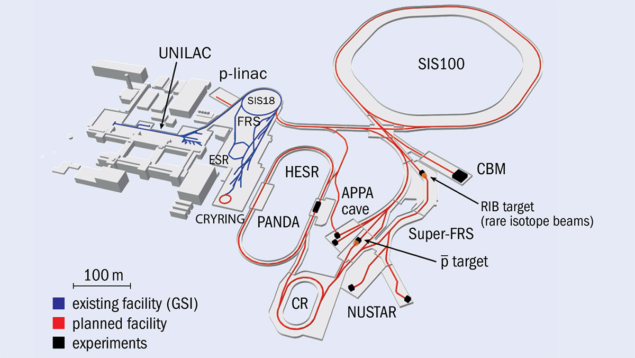
\includegraphics[width=\textwidth]{images/fair_sis100_diagram.jpg}
            \end{figure}
        \end{column}
        \begin{column}{0.5\textwidth}
            \begin{itemize}
                \item GSI (Gesellschaft für Schwerionenforschung) Helmholtzzentrum für Schwerionenforschung is a nuclear research facility in Darmstadt, Germany.
                \item The FAIR particle accelerator  facility is under construction (due 2027).
            \end{itemize}
        \end{column}
    \end{columns}
\end{frame}


\begin{frame}{Need for High-Performance Computing}
    \begin{columns}
        \begin{column}{0.5\textwidth}
            \begin{itemize}
                \item The rising complexity of nuclear physics experiments requires more computational power.
                \item Example: the CBM experiment will have an interaction rate of \SI{10}{\mega\hertz}.
            \end{itemize}
        \end{column}
        \begin{column}{0.5\textwidth}
            \begin{figure}
                \centering
                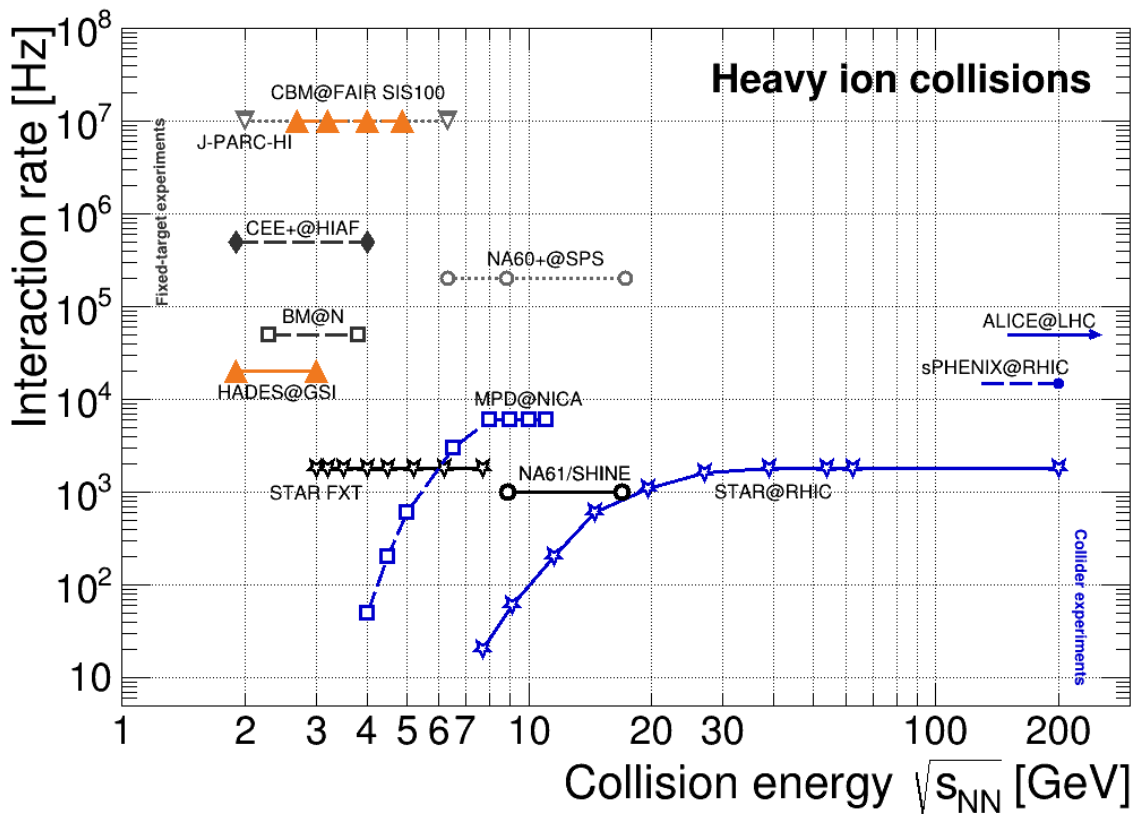
\includegraphics[width=\textwidth]{images/galatyuk_map_of_experiments.png}
                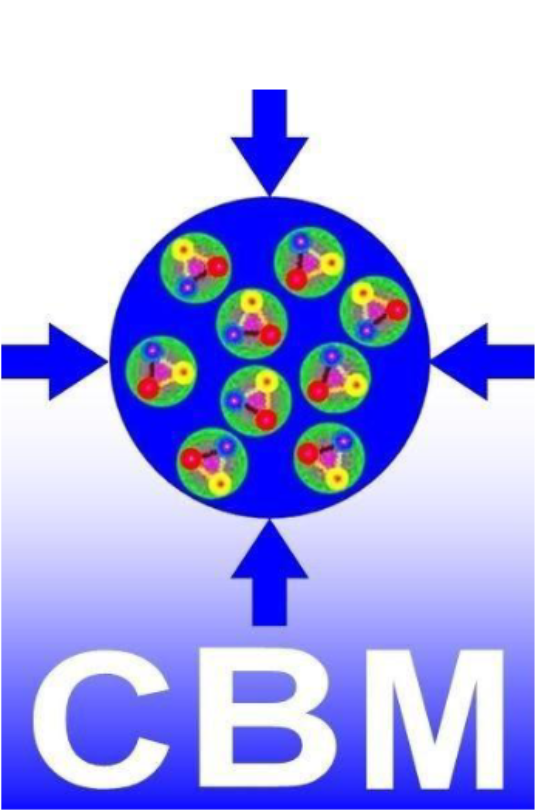
\includegraphics[width=0.2\textwidth]{images/cbm_logo.png}
            \end{figure}
        \end{column}
    \end{columns}
\end{frame}

\begin{frame}{Green Cube Data Center}
    \begin{columns}
        \begin{column}{0.5\textwidth}
            \begin{figure}
                \centering
                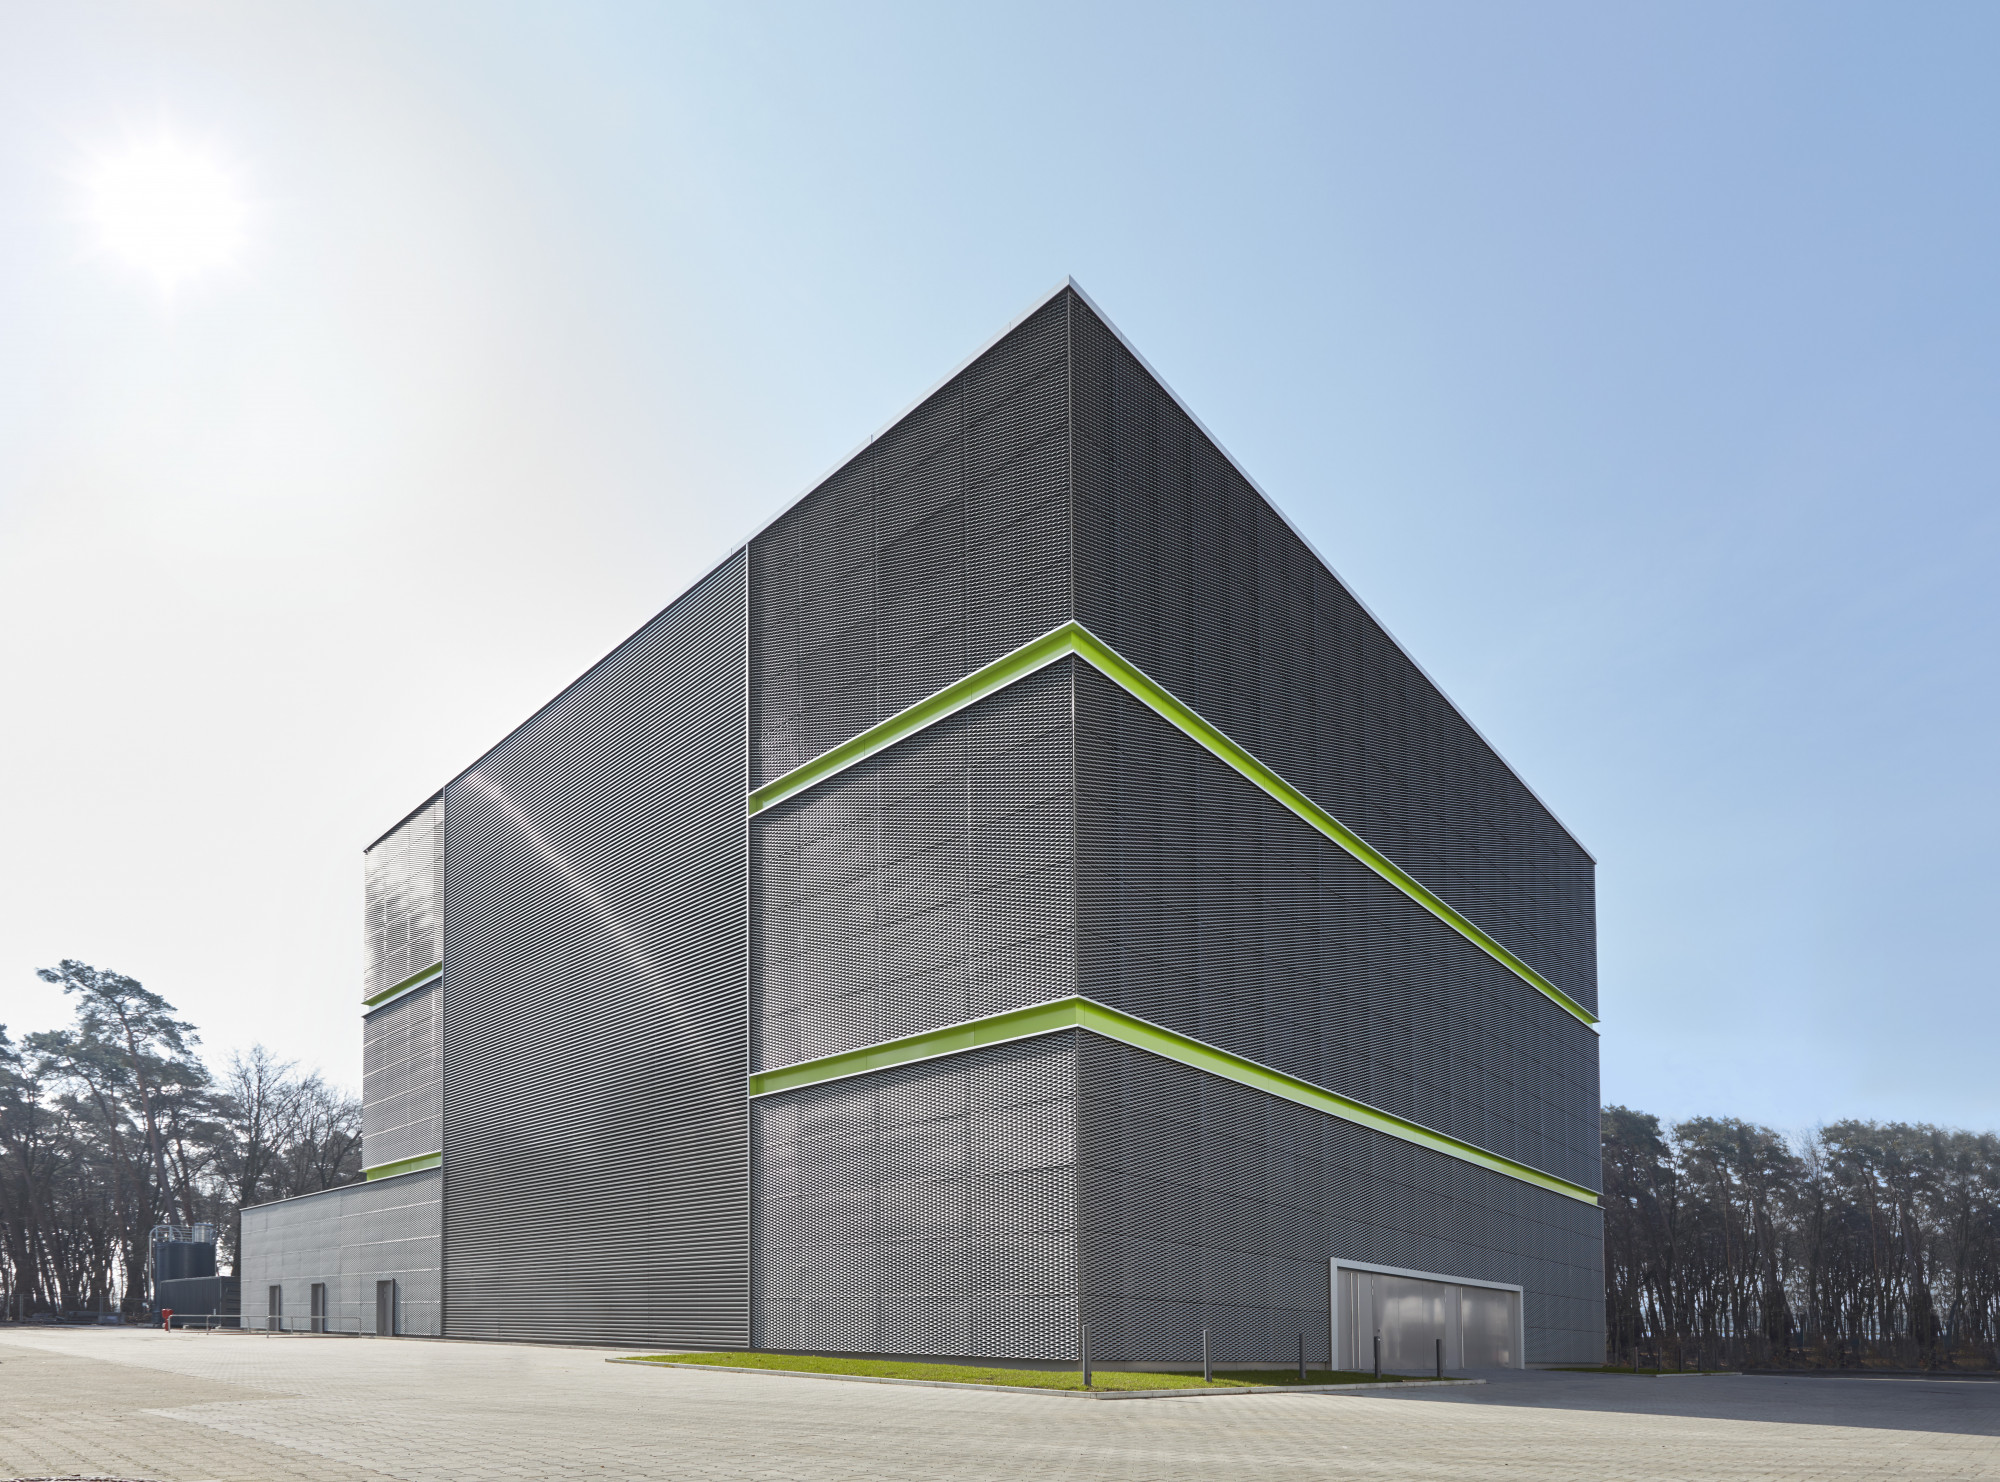
\includegraphics[width=\textwidth]{images/gsi_green_cube.jpg}
            \end{figure}
        \end{column}
        \begin{column}{0.5\textwidth}
            \begin{itemize}
                \item The Green Cube was built in 2015 as a solution to the growing computational needs of GSI (and in the future, FAIR).
                \item The investment totaled \num{12} million euros in construction costs and \num{21} million euros overall.
            \end{itemize}
        \end{column}
    \end{columns}
\end{frame}

% overall specs

% storage capabilities

% lustre

% working nodes

% slurm workload manager


\begin{frame}{}
    \centering
    \Large{Thank you for your attention}
\end{frame}

\end{document}
